\begin{figure}
    \centering
    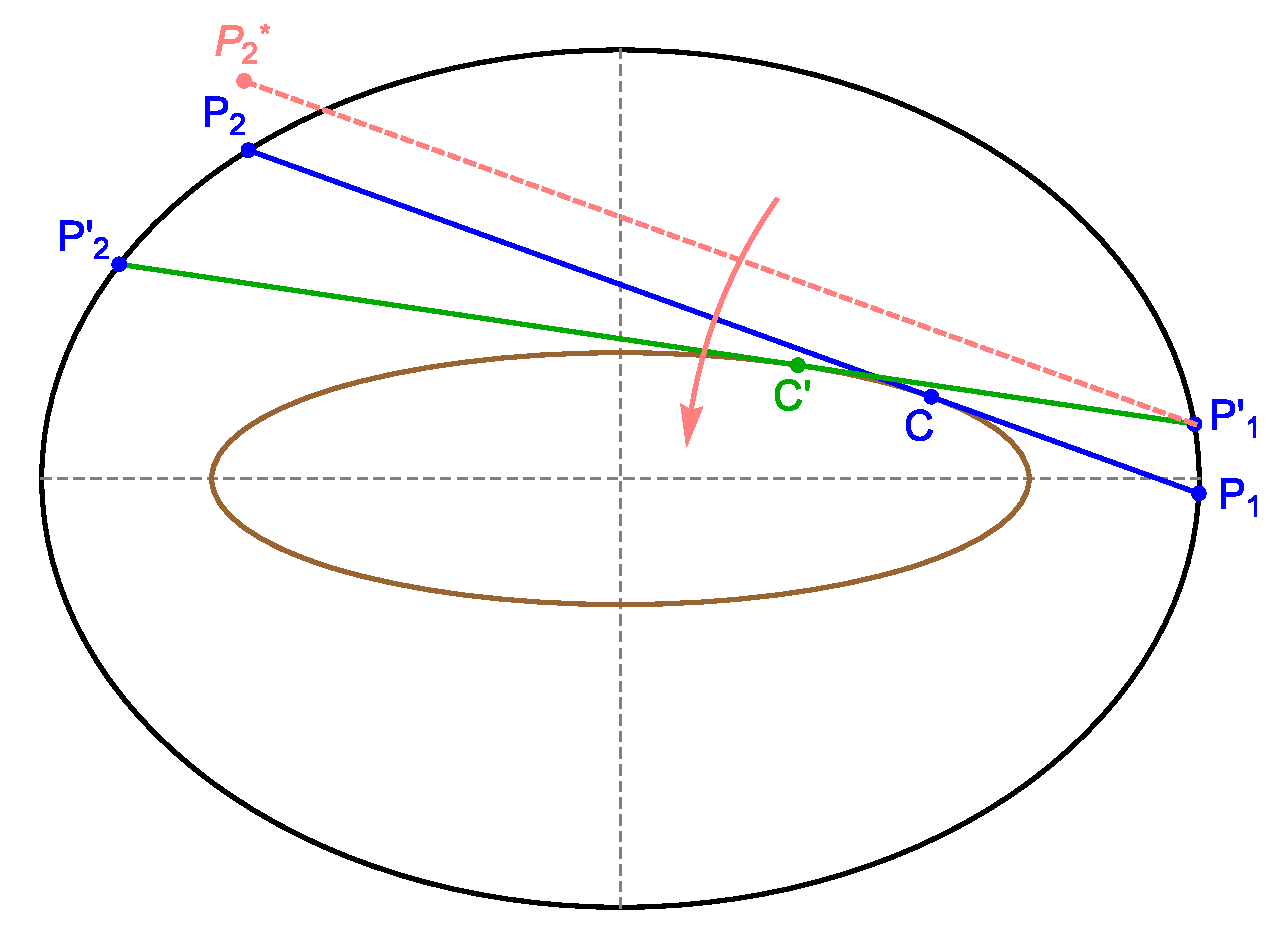
\includegraphics[width=.5\textwidth]{pics/1090_caustic_progress.eps}
    \caption{As one endpoint $P_1$ of a billiard trajectory is slid CCW to $P_1'$, its tangency point $C$ with the Caustic (brown) slides in the same direction to $C'$. This must be the case since $P_1'P_2'$ corresponds to a CCW rotation about $P_1'$ of segment $P_1'P_2^*$ (pink) parallel to $P_1P_2$ (see pink arrow). By convexity, said rotation will first touch the Caustic at $C'$, lying ``ahead'' of $C$. Repeating this for the $P_2P_3$ segment of a 3-periodic (not shown), it follows said vertices will move in the direction of $P_1$.}
    \label{fig:caustic-progress}
\end{figure}

\begin{figure}
    \centering
    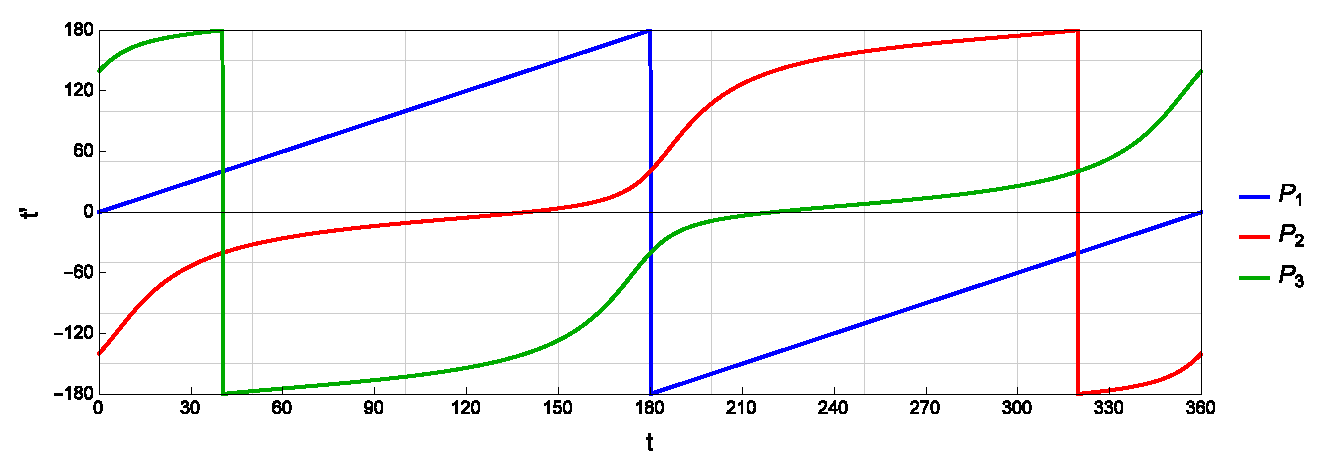
\includegraphics[width=.8\textwidth]{pics/1100_angular_progress_p1p2p3.eps}
    \caption{As $P_1(t)$ moves monotonically forward, so do $P_2(t)$ and $P_3(t)$, albeit with varying velocities with respect to $t$. In the text we mention an alternate parametrization (Poritsky-Lazutkin) under which the three lines would become straight.}
    \label{fig:ekg-p1p2p3}
\end{figure}


Let $P_1,P_2,P_3$ be the vertices of a\ 3-periodic, Appendix~\ref{app:vertices}.

\begin{proposition}
 If $P_1$ is slid along the EB in some direction, $P_2$ and $P_3$ will slide in the same direction. 
\end{proposition}

\begin{proof}
Consider the tangency point $C$ of $P_1P_2$ with the confocal Caustic, Figure~\ref{fig:caustic-progress}. Since this segment remains tangent to the Caustic for any choice of $P_1(t)$, a counterclockwise motion of $P_1(t)$ will cause $C$ to slide along the Caustic in the same direction, and therefore $P_2(t)$ will do the same.
\end{proof}

The simultaneous monotonic motion of 3-periodic vertices is shown in Figure~\ref{fig:ekg-p1p2p3}, note the non-linear progress of $P_2,P_3$. Alternatively, we could have linearized their motion using the so-called Poritsky-Lazutkin string length parameter $\eta$ for $C$ on the Caustic (Figure~\ref{fig:caustic-progress}) given by \cite{Poritsky1950, Lazutkin73, alexey19}:
%
$$
d\eta =  \kappa^{2/3}\,ds,
$$
%
\noindent where  $s$ is the arc length along the Caustic, and $\kappa$ is the curvature. 
Both $\eta$ and $s$ are related to the parameter $t$ on the billiard by elliptic functions. Adjusting conveniently with a constant factor, one has $\eta\equiv\eta+1$ and for any $\eta_o$ the other vertices correspond to  $\eta_o+1/3$ and $\eta_o+2/3$.

